\documentclass[preprint2]{aastex631}
\received{\today}
\shorttitle{Inside-Out Growth in the Milky Way Disc}
\graphicspath{{figures/}}

\usepackage{lipsum}
\usepackage{physics}
\usepackage{multirow}
\usepackage{xspace}
\usepackage{natbib}
\usepackage{fontawesome5}
\usepackage{xcolor}
\usepackage{wrapfig}
\usepackage[figuresright]{rotating}

% remove indents in footnotes
\usepackage[hang,flushmargin]{footmisc} 

\newcommand{\todo}[1]{{\color{red}{[TODO: #1}]}}
\newcommand{\needcite}{{\color{magenta}{(needs citation)}}}
\newcommand{\placeholder}[1]{{\color{gray} \lipsum[#1]}}

% custom function for adding units
\makeatletter
\newcommand{\unit}[1]{%
    \,\mathrm{#1}\checknextarg}
\newcommand{\checknextarg}{\@ifnextchar\bgroup{\gobblenextarg}{}}
\newcommand{\gobblenextarg}[1]{\,\mathrm{#1}\@ifnextchar\bgroup{\gobblenextarg}{}}
\makeatother

\begin{document}

\title{{\Large Inside-Out Growth in the Milky Way Disc [OUTLINE]}\\\vspace{0.15cm}ASTR 511 Final Project}

% affiliations
\newcommand{\UW}{Department of Astronomy, University of Washington, Seattle, WA, 98195}

\author[0000-0001-6147-5761]{Tom Wagg}
\affiliation{\UW}

\correspondingauthor{Tom Wagg}
\email{tomwagg@uw.edu}

% \begin{abstract}
%     todo
% \end{abstract}

\keywords{}

\section{Outline}
\textbf{Topic:} For my project I'm going to investigate the inside-out growth of galaxies, focussing specifically on the Milky Way. This is the idea that star formation in galaxies occurs first in the centre and builds outwards.

\textbf{Why I'm interested:} I'm particularly interested in looking into this as it went into a galaxy model for a paper I wrote on LISA predictions \citep{Wagg+2022} and I mostly trusted that it made sense without looking into it in detail. So I'd enjoy exploring 

\textbf{Specific papers:} The paper that I'll be using the centre my focus is \citet{Frankel+2019}, which conveniently addresses my exact topic. For the background information I think \citet{Fall+1980} could be fun to look into as one of the first papers predicting inside-out growth, whilst \citet{vanDokkum+2013} could be interesting to include for an example of observations of this effect. I think that the application of this concept in this paper \citep{Banerjee+2020} is very fun and I'm excited to read and talk about this. For future directions I think that the main limitation currently is the lack of precise ages for samples used in the stars in these studies and \citet{Hogg+2019} \textit{seems} to do some cool things combining APOGEE and Gaia to solve this, but I need to read that a bit more. I'm definitely also open to other paper suggestions!

\begin{figure}[htb]
    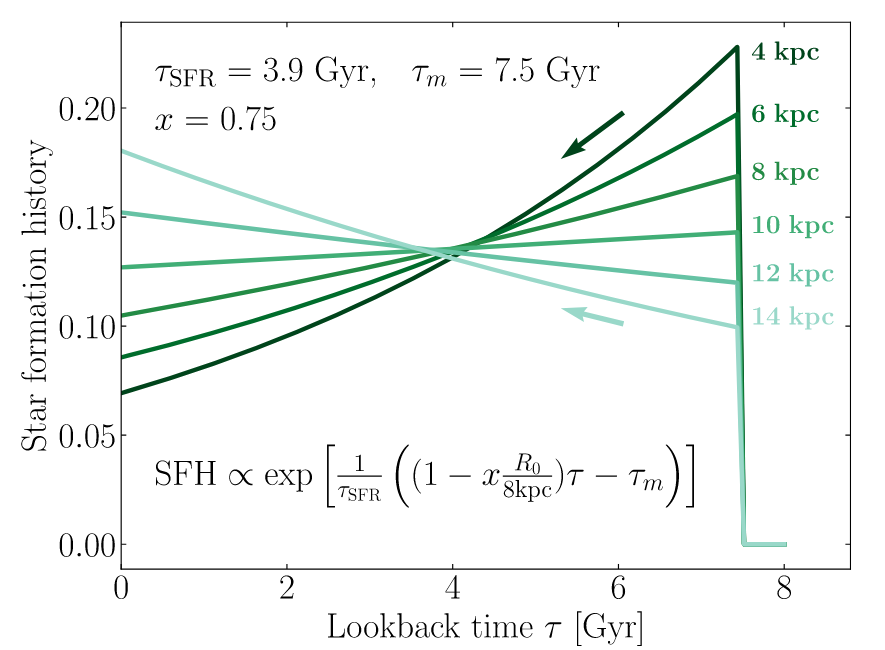
\includegraphics[width=\columnwidth]{frankel2019_fig5.png}
    \caption{\citet{Frankel+2019} Figure 5 showing the model for inside-out growth.}
\end{figure}

\bibliographystyle{aasjournal}
\bibliography{refs}{}

\end{document}